%************************************************
\chapter{System Model}\label{ch:model} 
%************************************************
%VWrite about the model and how it was built. 3D model of house was provided... Used software \texttt{Modelica}...
%Demonstate how model (acturately) predicts how the residential home behaves in real life to certain degree... Compare simulation to real life restults... Explain inaccuracies... which assumptions lead to these...
% Thermodynamic model, assumptions, constraints, design point conditions etc. 
% Equations 
% economic and ecological models. 

% \begin{flushright}{\slshape
%     The purpose of models is not to fit the data, but to sharpen the question} \\ \medskip
%     --- Samuel Karlin
% \end{flushright}

\section{Location} \label{sec:location}
The reference house that the building model is based off of a hipped dormer, two-storey residential house located in Belturbet, Cavan, a small town close to the Republic of Ireland and Northern Ireland border, about 125 kilometres from Dublin. The reference house lies at an elevation of 80 metres and is Easterly facing. The dwelling is located in a residential estate, and is thus classified as being located in an urban environment.

\section{Form and Fabric}
The reference model has a floor area of 160 square metres, 93 square metres of which are downstairs, i.e., ``exterior floor'', a gross roof area of 173 square metres and a total external wall surface area of 139 square metres. There are 21 exterior windows of varying sizes in total and thirteen rooms, seven downstairs and six upstairs. The ceiling height is a uniform 2.5 metres throughout the model. All rooms except for one were considered to be unconditioned, the exception being a very small box room on the ground floor which was interpreted to be a utility room of sorts. The void zones were also unconditioned. The building model geometry and thermal properties were created during previous works by \citeauthor{keogh_technical_2022}. A floor plan schematic can be seen in \cref{fig:floorplan}, showing the ground floor and first floor room layouts and windows. A 3D rendered model of the house can be seen in \cref{fig:3dmodel}. All building model data is contained in a \texttt{.idf}-file, an input data file interpretable by \texttt{EnergyPlus}. This file contains data about the geometry of the building, envelope construction, thermal and physical properties of the constructions, building and occupancy schedules, internal gains, outside air infiltration to void zones and various other data regarding the simulation process e.g., timestep. 

\begin{figure}[htb]
    \centering
    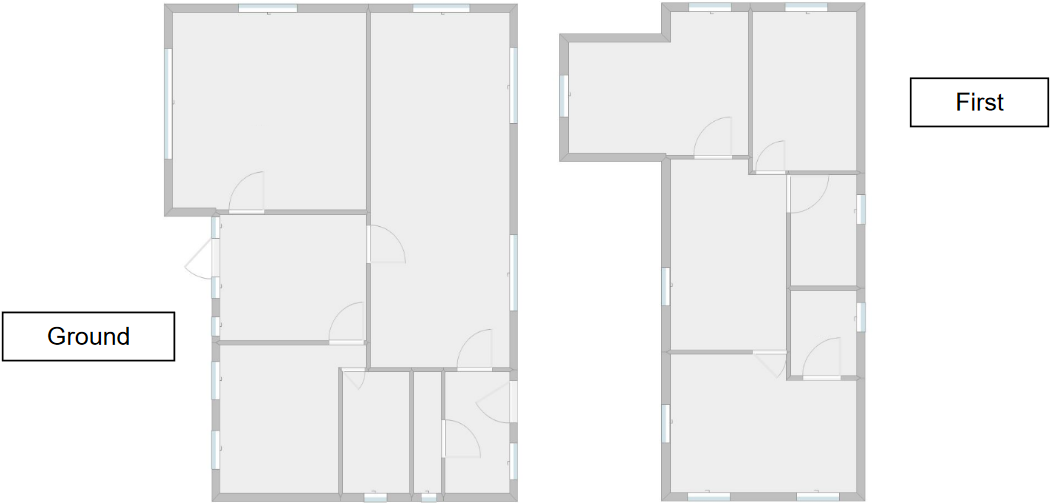
\includegraphics[width=0.75\linewidth]{dwellingFloorPlan}
    \caption{Dwelling Floor Plan}
    \label{fig:floorplan}
\end{figure}

\begin{figure}[htb]
    \centering
    %\includegraphics[width=0.7\linewidth]{3dmodel}
    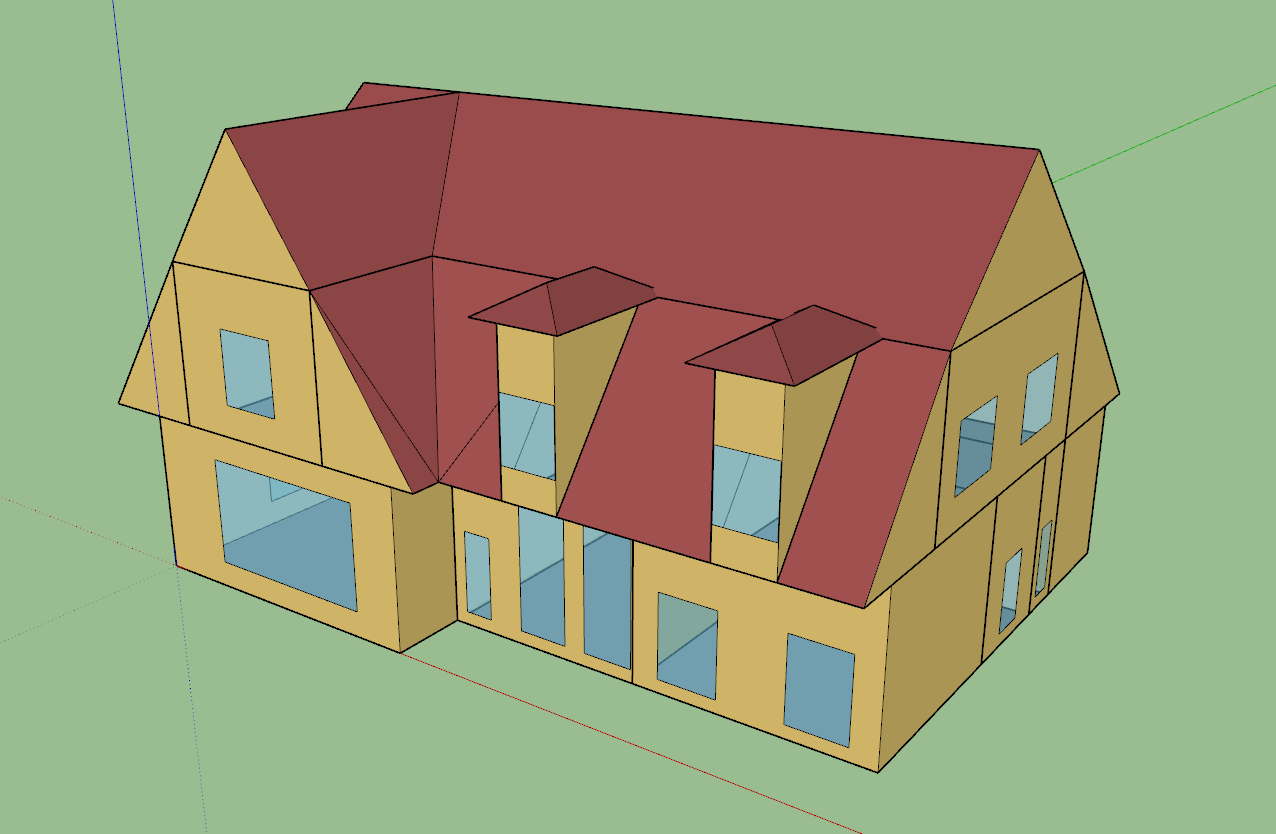
\includegraphics[width=0.7\linewidth]{Housepng.png}
    \caption[3D Model of Reference Building]{3D Model of Reference Building, rendered in \texttt{SketchUp} via the \texttt{Euclid} plugin.}
    \label{fig:3dmodel}
\end{figure}


\subsection{Thermal Properties of Constructions}

\begin{table}[htb]
    \footnotesize
    \centering
    \caption{Summary of $U$-Values}
    \label{tbl:uvalues}  
    \begin{tabular}{lccccc}\toprule
        \multicolumn{1}{c}{\multirow{2}{*}{\begin{tabular}[c]{@{}c@{}}Building \\ Model\end{tabular}}} & \multicolumn{4}{c}{\begin{tabular}[c]{@{}c@{}}$U$-Value\\ {[}\unit{\watt\per\square\meter\per\kelvin}{]}\end{tabular}} & \multirow{2}{*}{\begin{tabular}[c]{@{}c@{}}Infiltration\\ Rate\\ {[}\acs{ACPH}{]}\end{tabular}} \\ \cmidrule(lr){2-5}
        \multicolumn{1}{c}{} & \begin{tabular}[c]{@{}c@{}}Exterior\\ Wall\end{tabular} & \begin{tabular}[c]{@{}c@{}}Pitched\\ Roof\end{tabular} & \begin{tabular}[c]{@{}c@{}}Exterior\\ Floor\end{tabular} & \begin{tabular}[c]{@{}c@{}}Exterior\\ Glazing\end{tabular} &  \\ \midrule
        \begin{tabular}[c]{@{}l@{}}Minimal\\ Retrofit\end{tabular} & \num{0.31} & \num{0.16} & \num{0.25} & \num{2.15} & \num{0.8} %\\
        %\begin{tabular}[c]{@{}l@{}}Deep 
            %\\ Retrofit\end{tabular} & \num{0.18} & \num{0.16} & \num{0.18} & \num{1.39} & \num{0.5} 
            \\ \bottomrule   
    \end{tabular}
\end{table}

\subsubsection{Minimal Retrofit Model}
\cref{tbl:extwallconst} details the specifications of the exterior wall construction for the minimal retrofit model, from outside to inside. 
\begin{table}[htb]
    \footnotesize
    \centering
    \caption{Exterior Wall Construction}
    \label{tbl:extwallconst}
    \begin{tabular}{lcccc}
        \toprule
        Layer        & \multicolumn{1}{c}{\begin{tabular}[c]{@{}c@{}}Thickness \\ {[}m{]}\end{tabular}} & \multicolumn{1}{c}{\begin{tabular}[c]{@{}c@{}}Density \\ {[}\unit{\kilogram\per\cubic\meter}{]}\end{tabular}} & \multicolumn{1}{c}{\begin{tabular}[c]{@{}c@{}}Heat Capacity \\  {[}\unit{\joule\per\kilogram\per\kelvin}{]}\end{tabular}}  & \multicolumn{1}{c}{\begin{tabular}[c]{@{}c@{}}Conductivity \\   {[}\unit{\watt\per\meter\per\kelvin}{]}\end{tabular}} \\ \midrule
        Rainscreen   & \num{0.01}              & \num{7824}                & \num{500}                        & \num{30}                       \\
        Insulation   & \num{0.085}             & \num{43}                  & \num{1210}                       & \num{0.03}                     \\
        Air Cavity      & \num{0.15}              & $-$                  & $-$                      &  $-$                  \\
        Gypsum board & \num{0.019}             & \num{800}                 & \num{1090}                       & \num{0.16}                     \\
        \bottomrule
    \end{tabular}
\end{table}

\cref{tbl:extfloorconst} details the specifications of the exterior floor construction for the minimal retrofit model, from top to bottom. The exterior floor is the floor which lays on top of the foundations and therefore conducts heat from the inside of the house to the ground. It consists of concrete at the bottom, insulation board, an air cavity and floor tiles on top.

\begin{table}[htb]
    \footnotesize
    \centering
    \caption{Exterior Floor Construction}
    \label{tbl:extfloorconst}
    \begin{tabular}{lcccc}
        \toprule
        Layer        & \multicolumn{1}{c}{\begin{tabular}[c]{@{}c@{}}Thickness \\ {[}m{]}\end{tabular}} & \multicolumn{1}{c}{\begin{tabular}[c]{@{}c@{}}Density \\ {[}\unit{\kilogram\per\cubic\meter}{]}\end{tabular}} & \multicolumn{1}{c}{\begin{tabular}[c]{@{}c@{}}Heat Capacity \\  {[}\unit{\joule\per\kilogram\per\kelvin}{]}\end{tabular}}  & \multicolumn{1}{c}{\begin{tabular}[c]{@{}c@{}}Conductivity \\   {[}\unit{\watt\per\meter\per\kelvin}{]}\end{tabular}} \\ \midrule
        Acoustic Tile   & \num{0.0191}            & \num{368}                 & \num{590}                        & \num{0.06}                     \\
        Air Cavity      & \num{0.15}              & $-$                  & $-$                      &  $-$                  \\
        Insulation      & \num{0.085}             & \num{43}                  & \num{1210}                       & \num{0.03}                     \\
        Concrete        & \num{0.1016}             & \num{1280}                 & \num{840}                       & \num{0.53}                     \\
        \bottomrule
    \end{tabular}
\end{table}


\cref{tbl:pitchroofconst} details the specifications of the pitched roof construction for the minimal retrofit model, from outside to inside. This construction is applied to the bulk of the roof and consists of clay tile, an air cavity, insulation board and then plasterboard.

\begin{table}[htb]
    \footnotesize
    \centering
    \caption{Pitched Roof Construction}
    \label{tbl:pitchroofconst}
    \begin{tabular}{lcccc}
        \toprule
        Layer        & \multicolumn{1}{c}{\begin{tabular}[c]{@{}c@{}}Thickness \\ {[}m{]}\end{tabular}} & \multicolumn{1}{c}{\begin{tabular}[c]{@{}c@{}}Density \\ {[}\unit{\kilogram\per\cubic\meter}{]}\end{tabular}} & \multicolumn{1}{c}{\begin{tabular}[c]{@{}c@{}}Heat Capacity \\  {[}\unit{\joule\per\kilogram\per\kelvin}{]}\end{tabular}}  & \multicolumn{1}{c}{\begin{tabular}[c]{@{}c@{}}Conductivity \\   {[}\unit{\watt\per\meter\per\kelvin}{]}\end{tabular}} \\ \midrule
        Clay Tile   & \num{0.025}            & \num{1900}                 & \num{800}                        & \num{0.84}                     \\
        Air Cavity      & \num{0.15}              & $-$                  & $-$                      &  $-$                  \\
        Insulation      & \num{0.162}            & \num{43}                  & \num{1210}                       & \num{0.03}                     \\
        Gypsum board & \num{0.019}             & \num{800}                 & \num{1090}                       & \num{0.16}                     \\
        \bottomrule
    \end{tabular}
\end{table}

The dormer roof provides no insulation and is only in place to protect the inside spaces from wind and rain. Its specifications can be read in \cref{tbl:dormerroofconst}
\begin{table}[htb]
    \footnotesize
    \centering
    \caption{Hipped Dormer Roof Construction}
    \label{tbl:dormerroofconst}
    \begin{tabular}{lcccc}
        \toprule
        Layer        & \multicolumn{1}{c}{\begin{tabular}[c]{@{}c@{}}Thickness \\ {[}m{]}\end{tabular}} & \multicolumn{1}{c}{\begin{tabular}[c]{@{}c@{}}Density \\ {[}\unit{\kilogram\per\cubic\meter}{]}\end{tabular}} & \multicolumn{1}{c}{\begin{tabular}[c]{@{}c@{}}Heat Capacity \\  {[}\unit{\joule\per\kilogram\per\kelvin}{]}\end{tabular}}  & \multicolumn{1}{c}{\begin{tabular}[c]{@{}c@{}}Conductivity \\   {[}\unit{\watt\per\meter\per\kelvin}{]}\end{tabular}} \\ \midrule
        Clay Tile   & \num{0.025}            & \num{1900}                 & \num{800}                        & \num{0.84}                     \\
        Air Cavity      & \num{0.15}              & $-$                  & $-$                      &  $-$                  \\
        Roofing Felt      & \num{0.005}            & \num{960}                  & \num{837}                      & \num{0.19}                    \\
        \bottomrule
    \end{tabular}
\end{table}

\begin{table}[htb]
    \footnotesize
    \centering
    \caption{External Glazing Construction}
    \label{tbl:glazingconst}
    \begin{tabular}{lccc}
        \toprule
        Layer        & \multicolumn{1}{c}{\begin{tabular}[c]{@{}c@{}}Thickness \\ {[}m{]}\end{tabular}} & \multicolumn{1}{c}{\begin{tabular}[c]{@{}c@{}}Transmittance \\ {[}\unit{\kilogram\per\cubic\meter}{]}\end{tabular}}  & \multicolumn{1}{c}{\begin{tabular}[c]{@{}c@{}}Conductivity \\   {[}\unit{\watt\per\meter\per\kelvin}{]}\end{tabular}} \\ \midrule
        Inner Pane   & \num{0.003}            & \num{0.783}                 & \num{0.4}                                         \\
        Argon Gas      & \num{0.20}              & $-$                  & $-$                                   \\
        Outer Pane     & \num{0.003}            & \num{0.783}                  & \num{0.4}                                    \\
        \bottomrule
    \end{tabular}
\end{table}

% \subsubsection{Deep Retrofit Model}
% During the deep retrofit process, the external wall, exposed floor and external glazing constructions are upgraded to conform to the Building Regulations Part L 2022. The infiltration rate was also decreased to 0.5 \ac{ACPH} due to leakiness being heavily reduced.

% \begin{table}[htb]
%     \footnotesize
%     \centering
%     \caption{External Glazing Construction (Deep Retrofit)}
%     \label{tbl:deepglazingconst}
%     \begin{tabular}{lccc}
%         \toprule
%         Layer        & \multicolumn{1}{c}{\begin{tabular}[c]{@{}c@{}}Thickness \\ {[}m{]}\end{tabular}} & \multicolumn{1}{c}{\begin{tabular}[c]{@{}c@{}}Transmittance \\ {[}\unit{\kilogram\per\cubic\meter}{]}\end{tabular}}  & \multicolumn{1}{c}{\begin{tabular}[c]{@{}c@{}}Conductivity \\   {[}\unit{\watt\per\meter\per\kelvin}{]}\end{tabular}} \\ \midrule
%         Inner Pane   & \num{0.003}            & \num{0.783}                 & \num{0.4}                                         \\
%         Argon Gas      & \num{0.20}              & $-$                  & $-$                                   \\
%         Middle Pane   & \num{0.003}            & \num{0.783}                 & \num{0.4}                                         \\
%         Argon Gas      & \num{0.20}              & $-$                  & $-$                                   \\
%         Outer Pane     & \num{0.003}            & \num{0.783}                  & \num{0.4}                                    \\
%         \bottomrule
%     \end{tabular}   
% \end{table}

% \begin{table}[htb]
%     \footnotesize
%     \centering
%     \caption{Exterior Floor Construction}
%     \label{tbl:deepextfloorconst}
%     \begin{tabular}{lcccc}
%         \toprule
%         Layer        & \multicolumn{1}{c}{\begin{tabular}[c]{@{}c@{}}Thickness \\ {[}m{]}\end{tabular}} & \multicolumn{1}{c}{\begin{tabular}[c]{@{}c@{}}Density \\ {[}\unit{\kilogram\per\cubic\meter}{]}\end{tabular}} & \multicolumn{1}{c}{\begin{tabular}[c]{@{}c@{}}Heat Capacity \\  {[}\unit{\joule\per\kilogram\per\kelvin}{]}\end{tabular}}  & \multicolumn{1}{c}{\begin{tabular}[c]{@{}c@{}}Conductivity \\   {[}\unit{\watt\per\meter\per\kelvin}{]}\end{tabular}} \\ \midrule
%         Acoustic Tile   & \num{0.0191}            & \num{368}                 & \num{590}                        & \num{0.06}                     \\
%         Air Cavity      & \num{0.15}              & $-$                  & $-$                      &  $-$                  \\
%         Insulation      & \num{0.085}             & \num{43}                  & \num{1210}                       & \num{0.03}                     \\
%         Concrete        & \num{0.1016}             & \num{1280}                 & \num{840}                       & \num{0.53}                     \\
%         \bottomrule
%     \end{tabular}
% \end{table}

% \begin{table}[htb]
%     \footnotesize
%     \centering
%     \caption{Exterior Wall Construction}
%     \label{tbl:deepextwallconst}
%     \begin{tabular}{lcccc}
%         \toprule
%         Layer        & \multicolumn{1}{c}{\begin{tabular}[c]{@{}c@{}}Thickness \\ {[}m{]}\end{tabular}} & \multicolumn{1}{c}{\begin{tabular}[c]{@{}c@{}}Density \\ {[}\unit{\kilogram\per\cubic\meter}{]}\end{tabular}} & \multicolumn{1}{c}{\begin{tabular}[c]{@{}c@{}}Heat Capacity \\  {[}\unit{\joule\per\kilogram\per\kelvin}{]}\end{tabular}}  & \multicolumn{1}{c}{\begin{tabular}[c]{@{}c@{}}Conductivity \\   {[}\unit{\watt\per\meter\per\kelvin}{]}\end{tabular}} \\ \midrule
%         Rainscreen   & \num{0.01}              & \num{7824}                & \num{500}                        & \num{30}                       \\
%         Insulation   & \num{0.085}             & \num{43}                  & \num{1210}                       & \num{0.03}                     \\
%         Air Cavity      & \num{0.15}              & $-$                  & $-$                      &  $-$                  \\
%         Gypsum board & \num{0.019}             & \num{800}                 & \num{1090}                       & \num{0.16}                     \\
%         \bottomrule
%     \end{tabular}
% \end{table}



 

\section{Schedules, Equipment and Internal Gains}
Internal gains in the context of an energy building simulation of a residential home refers to the heat generated within the envelope by people, appliances, and lighting.

People generate heat through their activities and body heat, while appliances generate heat through their operation. Lighting generates heat due to the inefficiencies in converting electricity into light, and light ultimately being converted to heat energy.

In energy building simulation, internal gains are important to consider because they can significantly affect the energy balance of the building. If the internal gains are high, the building may require less heating, which can lead to energy savings. Conversely, if the internal gains are low, the building may require more heating, which can lead to increased energy consumption and costs. \cite{buttitta_high-temporal_2020}

Internal gains are typically modelled as a heat input to the building, which is then factored into the overall energy balance of the building. The magnitude of internal gains is typically calculated based on the number of occupants, the types and number of appliances, and the lighting levels in the building.

\subsection{Occupancy Gains}
The magnitude of these gains depends on factors such as the number of occupants, their activity levels, and the duration of their stay in the building. It was decided that a house of the size of the reference home was sized for a total of four persons. 

In order to accurately model occupancy gains in a \ac{BEM}, it is important to use typical occupancy profiles in conjunction with typical metabolic rates for different tasks. A typical occupancy profile is a representation of the number of occupants in the building over time, while a typical metabolic rate is a measure of the heat generated by a person due to their physical activity. Different tasks require different amounts of energy, and therefore result in different levels of heat generation. For example, a person sitting quietly may have a lower metabolic rate than someone performing strenuous physical activity.

\citeauthor{buttitta_high-temporal_2020} \cite{buttitta_high-temporal_2020} developed a stochastic occupancy model which generates hourly occupancy schedules for up to five different types of occupancy profiles of residential buildings for an entire year, based off of data gathered from London, UK. For this thesis, an occupancy profile was chosen which represented the largest share of the population, and two schedules were drawn, one for the weekdays and one for the weekends. These schedules depict the number of persons occupying the dwelling at each hour of the day, and the weekday schedule is detailed in \cref{tbl:occupancysched}. The table shows the fraction of the (four) occupants in the home at the corresponding time interval. For the weekend schedule, it was assumed that all occupants remain home all day.

\begin{table}[htb]
    \centering
    \caption{Weekday Occupancy Schedules}
    \label{tbl:occupancysched}
    \begin{tabular}
        {lcr}
        \toprule
        Time & Fraction of Occupants \\
        \midrule
        \num[parse-numbers=false]{00}:\num[parse-numbers=false]{00} $\rightarrow$ \num[parse-numbers=false]{06}:\num[parse-numbers=false]{50} & \num{1.0}\\
        \num[parse-numbers=false]{06}:\num[parse-numbers=false]{50} $\rightarrow$ \num[parse-numbers=false]{07}:\num[parse-numbers=false]{30} & \num{0.75}\\
        \num[parse-numbers=false]{07}:\num[parse-numbers=false]{30} $\rightarrow$ \num[parse-numbers=false]{08}:\num[parse-numbers=false]{20} & \num{0.5}\\
        \num[parse-numbers=false]{08}:\num[parse-numbers=false]{20} $\rightarrow$ \num[parse-numbers=false]{18}:\num[parse-numbers=false]{20} & \num{0.0}\\
        \num[parse-numbers=false]{18}:\num[parse-numbers=false]{20} $\rightarrow$ \num[parse-numbers=false]{24}:\num[parse-numbers=false]{00} & \num{1.0}\\
        \bottomrule
    \end{tabular}
\end{table}

\citetitle{ashrae_ansiashrae_2010} \cite{ashrae_ansiashrae_2010} details the metabolic rate of people performing various tasks, given in Met units, as well as watts per square metre. An activity level schedule was quasi-arbitrarily assembled and is detailed in \cref{tbl:activitysched}. The table, which is very similar to the occupancy schedule in nature, shows the metabolic rate in watts per square metre for the corresponding time interval. \texttt{EnergyPlus} takes this metabolic rate and multiplies it by a value of \qty{1.8}{\square\meter}, deemed to be the standard surface area of a typical adult. As a reference, a rate of \qty{40}{\watt\per\square\meter} corresponds to sleeping, \qtyrange{50}{90}{\watt\per\square\meter} are non-strenuous activities such as lounging, reading, etc. and above \qty{100}{\watt\per\square\meter} corresponds to activities such as walking briskly and beyond.
 
\begin{table}[htb]
    \centering
    \caption{Activity Schedules}
    \label{tbl:activitysched}
    \begin{subtable}[t]{0.485\linewidth}
        %\centering
        \caption{Weekday Activity Schedule}
        \begin{tabular}
        {lr}
        \toprule
        Time & \multicolumn{1}{c}{\begin{tabular}[c]{@{}c@{}}Metabolic\\ rate\\ {[}\unit{\watt\per\square\meter}{]}\end{tabular}}   \\
        \midrule
        \num[parse-numbers=false]{00}:\num[parse-numbers=false]{00} $\rightarrow$ \num[parse-numbers=false]{06}:\num[parse-numbers=false]{50} & \num{40}\\
        \num[parse-numbers=false]{06}:\num[parse-numbers=false]{50} $\rightarrow$ \num[parse-numbers=false]{08}:\num[parse-numbers=false]{20} & \num{120}\\
        \num[parse-numbers=false]{08}:\num[parse-numbers=false]{20} $\rightarrow$ \num[parse-numbers=false]{18}:\num[parse-numbers=false]{20} & \num{0.0}\\
        \num[parse-numbers=false]{18}:\num[parse-numbers=false]{20} $\rightarrow$ \num[parse-numbers=false]{22}:\num[parse-numbers=false]{00} & \num{120}\\
        \num[parse-numbers=false]{20}:\num[parse-numbers=false]{00} $\rightarrow$ \num[parse-numbers=false]{23}:\num[parse-numbers=false]{10} & \num{75}\\
        \num[parse-numbers=false]{23}:\num[parse-numbers=false]{10} $\rightarrow$ \num[parse-numbers=false]{24}:\num[parse-numbers=false]{00} & \num{40}\\
        \bottomrule
    \end{tabular}
    \end{subtable}%
    \hfill
    \begin{subtable}[t]{0.485\linewidth}
        %\centering
        \caption{Weekend Activity Schedule}
        \begin{tabular}
        {lr}
        \toprule
        Time & \multicolumn{1}{c}{\begin{tabular}[c]{@{}c@{}}Metabolic\\ rate\\ {[}\unit{\watt\per\square\meter}{]}\end{tabular}} \\
        \midrule
        \num[parse-numbers=false]{00}:\num[parse-numbers=false]{00} $\rightarrow$ \num[parse-numbers=false]{01}:\num[parse-numbers=false]{00} & \num{75}\\
        \num[parse-numbers=false]{01}:\num[parse-numbers=false]{00} $\rightarrow$ \num[parse-numbers=false]{07}:\num[parse-numbers=false]{20} & \num{40}\\
        \num[parse-numbers=false]{07}:\num[parse-numbers=false]{20} $\rightarrow$ \num[parse-numbers=false]{09}:\num[parse-numbers=false]{30} & \num{75}\\
        \num[parse-numbers=false]{09}:\num[parse-numbers=false]{30} $\rightarrow$ \num[parse-numbers=false]{24}:\num[parse-numbers=false]{00} & \num{120}\\
        \num[parse-numbers=false]{20}:\num[parse-numbers=false]{00} $\rightarrow$ \num[parse-numbers=false]{23}:\num[parse-numbers=false]{10} & \num{75}\\
        \num[parse-numbers=false]{23}:\num[parse-numbers=false]{10} $\rightarrow$ \num[parse-numbers=false]{24}:\num[parse-numbers=false]{00} & \num{40}\\
        \bottomrule
        \end{tabular}
    \end{subtable}%
\end{table}

\subsection{Lighting}
In the past, internal gains from lighting used to be a significant contributor to the overall heat load of buildings. This was largely due to the widespread use of inefficient incandescent light bulbs, which generated a significant amount of heat as a byproduct of their operation. In fact, it was not uncommon for incandescent bulbs to emit more heat than light, resulting in a significant waste of energy and contributing to higher cooling loads in buildings.

However, with the gradual adoption of more efficient lighting technologies such as LED bulbs, internal gains from lighting have become much less of a concern. LED bulbs are significantly more efficient than incandescent bulbs, converting a higher percentage of their energy input into light rather than heat. This means that they generate far less waste heat, resulting in lower cooling loads and reduced energy consumption. \citefield{ISO17772}{shorttitle} presents lighting schedules and load density profiles for single family residential homes, and are reproduced in \cref{tbl:lightandequip}. 

\subsection{Plug Loads and Equipment}
Plug loads in a residential home refer to the energy consumed by appliances and devices that are plugged into electrical outlets, such as televisions, computers, and kitchen appliances. Equipment internal gains in a residential home refer to the heat generated by the operation of various equipment and appliances, such as refrigerators, ovens, and water heaters. This heat can contribute to the overall heat load of the home, particularly during periods of high use. \citefield{ISO17772}{shorttitle} gives details regarding standards for schedules and load density profiles for equipment gains and plug loads, and is reproduced in \cref{tbl:lightandequip}, showing the fraction of the load thought to be ``active'' at the corresponding time. The nominal lighting load is given to be \qty{2.07}{\watt\per\square\meter} and nominal equipment load is given to be \qty{1.92}{\watt\per\square\meter}

\begin{table}[htb]
    \centering
    \caption{Lighting, Plug Loads and Equipment Gains Schedules and Load Densities \cite{ISO17772}}
    \label{tbl:lightandequip}
    \begin{subtable}[t]{0.485\linewidth}
        %\centering
        \caption{Lighting Schedule}
        \begin{tabular}
        {lcr}
        \toprule
        Time & \multicolumn{1}{c}{\begin{tabular}[c]{@{}c@{}}Fraction of\\ nom. value\end{tabular}}  \\
        \midrule
        \num[parse-numbers=false]{00}:\num[parse-numbers=false]{00} $\rightarrow$ \num[parse-numbers=false]{07}:\num[parse-numbers=false]{00} & \num{0.251}\\
        \num[parse-numbers=false]{07}:\num[parse-numbers=false]{00} $\rightarrow$ \num[parse-numbers=false]{11}:\num[parse-numbers=false]{00} & \num{0.749}\\
        \num[parse-numbers=false]{17}:\num[parse-numbers=false]{00} $\rightarrow$ \num[parse-numbers=false]{23}:\num[parse-numbers=false]{00} & \num{0.251}\\
        \num[parse-numbers=false]{23}:\num[parse-numbers=false]{00} $\rightarrow$ \num[parse-numbers=false]{24}:\num[parse-numbers=false]{00} & \num{0.749}\\
        \bottomrule
    \end{tabular}
    \end{subtable}
    \hfill
    \begin{subtable}[t]{0.485\linewidth}
        \centering
        \caption{Equipment Schedule}
        \begin{tabular}
        {lcr}
        \toprule
        Time & \multicolumn{1}{c}{\begin{tabular}[c]{@{}c@{}}Fraction of\\ nom. value\end{tabular}} \\
        \midrule
        \num[parse-numbers=false]{00}:\num[parse-numbers=false]{00} $\rightarrow$ \num[parse-numbers=false]{08}:\num[parse-numbers=false]{00} & \num{0.625}\\
        \num[parse-numbers=false]{08}:\num[parse-numbers=false]{00} $\rightarrow$ \num[parse-numbers=false]{10}:\num[parse-numbers=false]{00} & \num{0.875}\\
        \num[parse-numbers=false]{10}:\num[parse-numbers=false]{00} $\rightarrow$ \num[parse-numbers=false]{12}:\num[parse-numbers=false]{00} & \num{0.625}\\
        \num[parse-numbers=false]{12}:\num[parse-numbers=false]{00} $\rightarrow$ \num[parse-numbers=false]{16}:\num[parse-numbers=false]{00} & \num{0.750}\\
        \num[parse-numbers=false]{16}:\num[parse-numbers=false]{00} $\rightarrow$ \num[parse-numbers=false]{18}:\num[parse-numbers=false]{00} & \num{0.625}\\
        \num[parse-numbers=false]{18}:\num[parse-numbers=false]{00} $\rightarrow$ \num[parse-numbers=false]{20}:\num[parse-numbers=false]{00} & \num{0.875}\\
        \num[parse-numbers=false]{20}:\num[parse-numbers=false]{00} $\rightarrow$ \num[parse-numbers=false]{22}:\num[parse-numbers=false]{00} & \num{1.0}\\
        \num[parse-numbers=false]{22}:\num[parse-numbers=false]{00} $\rightarrow$ \num[parse-numbers=false]{24}:\num[parse-numbers=false]{00} & \num{0.750}\\
        \bottomrule
        \end{tabular}
    \end{subtable}
\end{table}

\section{Heating System}
\begin{figure}[htb]
    \centering
    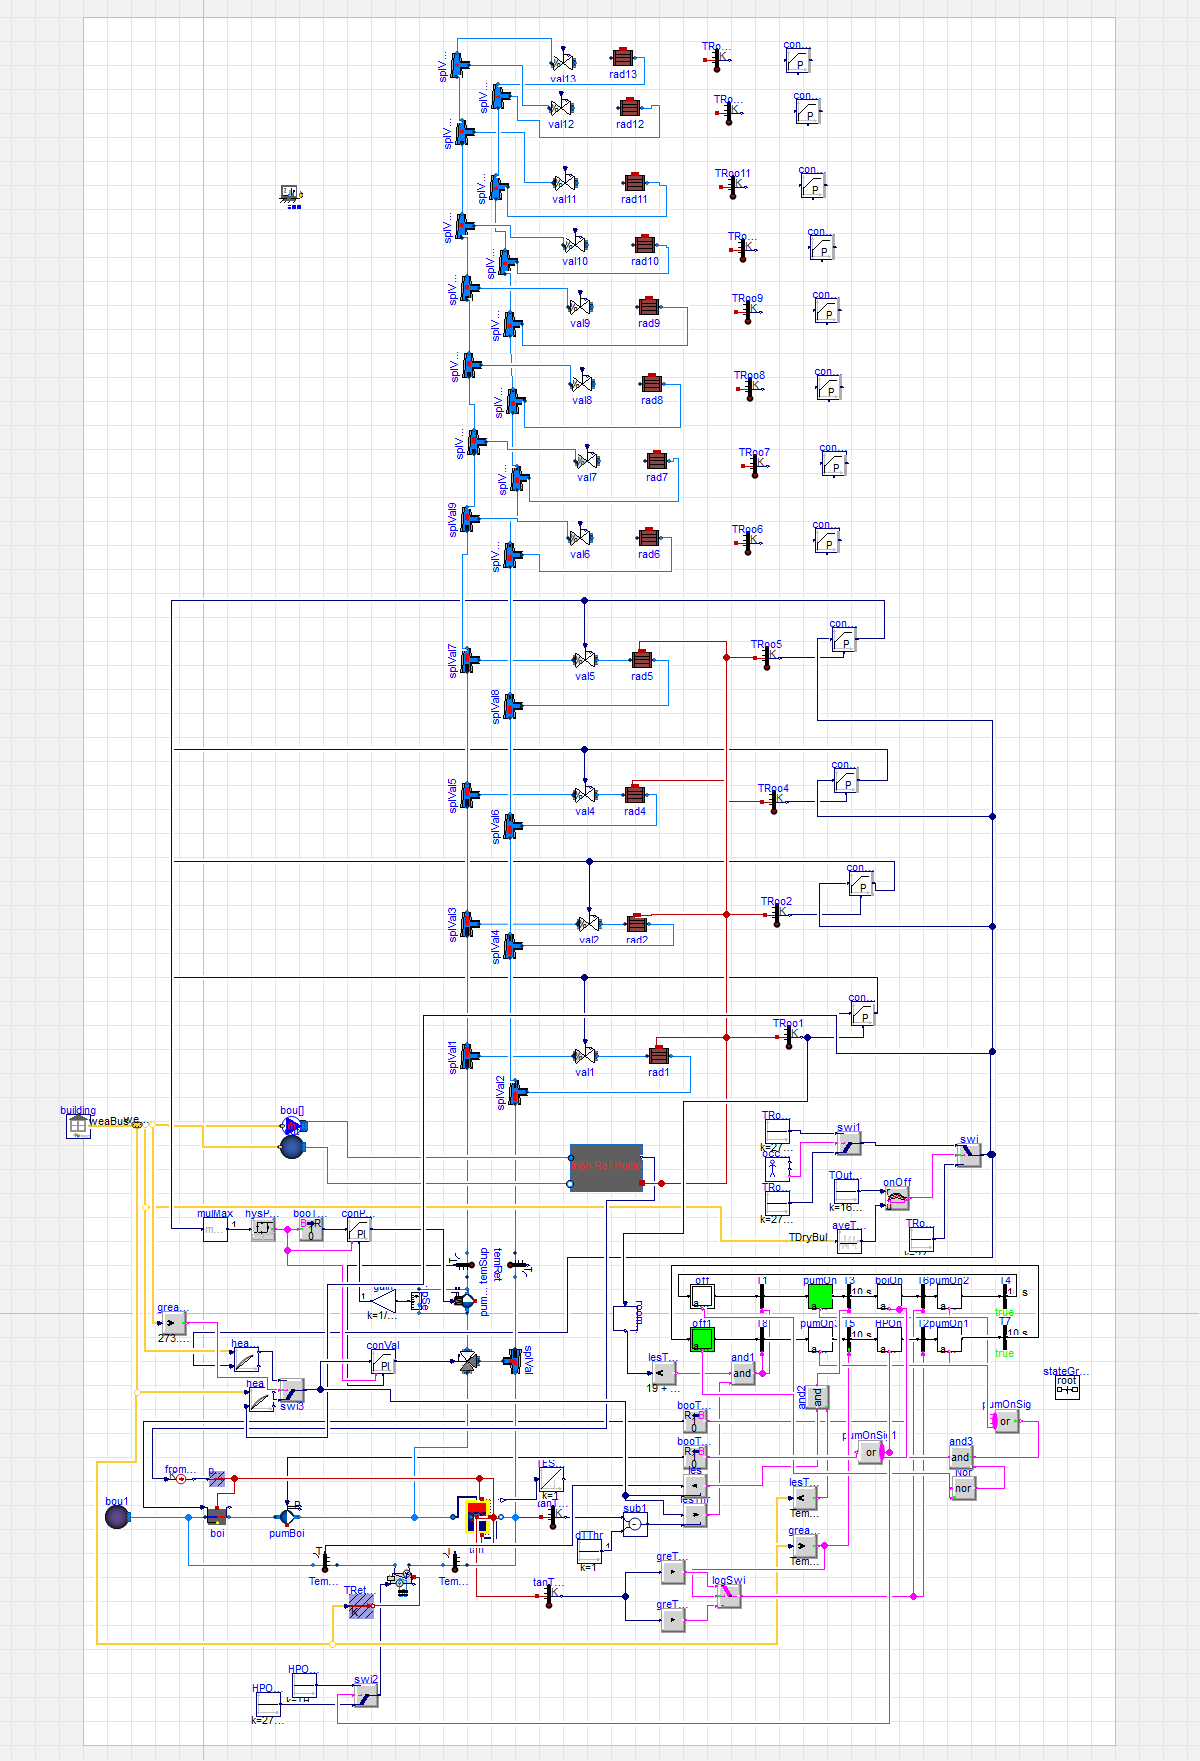
\includegraphics[width=0.8\linewidth]{ModelicaHHSDiagram}
    \caption{\modelica Diagram view of implemented system}
    \label{fig:modelicadiagram}
\end{figure}
\subsection{ASHP} \label{subsec:ashp}
The \ac{ASHP} model was imported from the IDEAS library \cite{jorissen_implementation_2018}.Performance table data obtained from Daikin for a low-temperature, modulating \ac{AWHP} was used in the modelling of the heat pump. By interpolating the data in the table, the model is able to determine the heating power, electricity usage, and \ac{COP} based on the condenser outlet temperature and the ambient temperature. The \HP has a nominal heating power of \qty{7177}{\watt} at a test condition of 2/\qty{35}{\celsius} (air/condenser temperature), with a \ac{COP} of 3.17 at this condition and a \ac{COP} of 2.44 at a test condition of 2/\qty{45}{\celsius} for full load operation. The heat pump can operate at leaving water temperatures up to \qty{55}{\celsius}.

The \ac{COP} of the \ac{AWHP} model is calculated by the ratio of heat energy transferred to the passing water to the electrical power used. This is given by \cref{eq:cop}. 

\begin{equation}
    \operatorname{COP}_\text{HP}=\frac{\dot{Q}_\text{H}}{\dot{W}_\text{elec}}\label{eq:cop}
\end{equation}

The \ac{SCOP} of the \HP is calculated by taking the ratio the total heat energy imparted to the water to the total electrical energy used by the \HP over the course of the year and is given by \cref{eq:scop}
\begin{equation}
    \operatorname{SCOP}_\text{HP}=\frac{Q_\text{H, tot}}{W_\text{elec, tot}}\label{eq:scop}
\end{equation}

The model uses modulation to introduce some hysteresis to avoid quick-succession, repeated on-off cycling. The \HP turns off when the modulation drops below 20\% and turns on when the modulation exceeds 35\%. Heat losses to the surroundings are taken into account to produce a dynamic model, all the while maintaining the performance as per Daikin's data \cite{daikin_altherma_tech_2006}.

\subsubsection{Frosting Modelling} \label{subsubsec:frostingmod}
The model provided by IDEAS library does not include frosting effects. Thus, a simple model for the repercussions of frosting on the \ac{ASHP} was developed in the \modelica model. A conditional timer block and greater-than-threshold block were used to identify whether the outdoor temperature had been less than \qty{2}{\celsius} for an aggregate of 60 minutes, resetting the timer only if the outdoor temperature had exceeded \qty{4}{\celsius} for a contiguous 5-minute period. If this 60-minute condition was met, the \ac{ASHP} was turned off, no matter the modulation level, for 10 minutes. This is intended to introduce a ``penalty'' to the \HP for operating under cold conditions. The approximate values were taken from \citeauthor{sandstrom_frosting_2021} \cite{sandstrom_frosting_2021}. To account for energy loss due to a reverse-cycling defrosting of the \HP, \qty{500000}{\joule} of energy was removed from the buffer tank. This figure was calculated using data from \citeauthor{sandstrom_frosting_2021} \cite{sandstrom_frosting_2021} and the 60\% defrosting efficiency figure mentioned in \cref{subsec:defrost}. 

\subsection{Radiators}
The \texttt{RadiatorEN442} radiator model from the Buildings library \cite{wetter_modelica_2014} was used. Each of the twelve conditioned rooms was assigned a radiator. The nominal heat flow for a radiator in room $i$ was determined by taking the nominal total heat flow of the system, $Q_\text{flow, nom}$ and multiplying it by the ratio of the volume of room $i$, $V_{\text{room, }i}$ to the total conditioned room volume, $V_\text{rooms, tot}$. The radiator model uses five discretised elements to perform a discretised element method heat transfer calculation. The model parameters were altered to only produce convective heat transfer to the room i.e., no radiative heat transfer as the \texttt{EnergyPlus} compatible \texttt{ThermalZone} model has no radiative heat input. The heat transfer was modelled with \cref{eq:radiatorheatrans} 


\begin{equation}
    Q_\text{c}^i=\operatorname{sign}(T^i-T_\text{a})(1-f_\text{rad})\frac{UA}{N}|T^i-T_\text{a}|^n\label{eq:radiatorheatrans}
\end{equation}

Where $T^i$ is the water temperature of the element, $T_\text{a}$ is the temperature of the air in the room, $f_\text{rad}$ is the fraction of the heat converted to radiation, set to zero in this model, $n$ is the exponent of heat transfer, set to 1.3, and $UA$ is the $UA$-value of the radiator which is numerically solved for the given nominal data values. 

\subsection{Thermal Storage Tank}
The thermal storage tank \texttt{Thermal.Storage} model from the Buildings library \cite{wetter_modelica_2014} was used in the \ac{HHS} model. The model uses ten stratified layers (\texttt{nSeg = 10}) to model to dynamics of the temperature gradient of the water within the tank. The storage tank was fixed to contain \qty{0.5}{\cubic\meter} of water, or \qty{500}{\litre}, with \qty{10}{\centi\meter} of insulation thickness and a height of \qty{1.7}{\meter}. The tank was assumed to be located in the aforementioned unconditioned room, with heat losses occurring from the tank to the room. Two temperature sensors are connected to the tank, one at the top of the water volume (volume index 1) and one at the bottom of the water volume (volume index \texttt{nSeg}). 

\subsection{Boiler}
The boiler model \texttt{BoilerPolynomial} from the Buildings library was utilised to model the natural gas boiler component of the \ac{HHS}. A constant efficiency of 90\% was used as this best matched the efficiency of the reference house boiler. A nominal mass flowrate of \qty{0.25}{\kilo\gram\per\second} was inputted, which had been calculated through \cref{eq:boiflowcalc}.

\begin{equation}
    \dot{m}_\text{boi, nom} = \frac{k\dot{Q}_\text{nom}}{\Delta T_\text{boi loop}  c_\text{water}} \label{eq:boiflowcalc}
\end{equation}
The coefficient $k$ is simply a scaling factor that affects the massflow rate and downstream variables.

The rate of heat produced by the fuel is calculated using \cref{eq:heatcombboi}, where $y \in [0\text{, }1]$ is the control signal, determined by the \ac{HHS} logic control outlined in \cref{fig:hhsflowchart}, $\dot{Q}_0$ is the nominal heating power, set to \qty{10}{\kilo\watt}, and $\eta_0$ is the nominal efficiency.
\begin{equation}
    \dot{Q}_\text{f} = y \frac{\dot{Q}_0}{\eta_0}\label{eq:heatcombboi}
\end{equation}
\cref{eq:heattofluid} determines the heat transferred to the passing water. $\eta$ is the efficiency at the at instantaneous operating temperature and $\dot{Q}_\text{amb} > 0 $ is the heat loss to the ambient. The boiler has a boundary condition of its heat port which is connected to the air of the unconditioned zone where the boiler is assumed to be installed.  
\begin{equation}
    \dot{Q} = \eta \dot{Q}_\text{f} - \dot{Q}_\text{amb}\label{eq:heattofluid}
\end{equation}

\cref{eq:massflowfuel} gives the mass flowrate and the volumetric flowrate of the fuel, where $h_\text{f}$ is the heating value of the fuel, and $\rho_\text{f}$ is the density of the fuel, \qty{845}{\kilo\gram\per\cubic\meter}. Since a condensing gas boiler is being used, the higher heating value of gas (\qty{4.26E7}{\joule\per\kilo\gram}) is being used.

 \begin{equation}
    \dot{m}_\text{f} =\frac{\dot{Q}_\text{f}}{h_\text{f}}\label{eq:massflowfuel}\text{\;\;\; ; \;\;\;} \dot{V}_\text{f} =\frac{\dot{m}_\text{f}}{\rho_\text{f}}
 \end{equation}


\subsection{Heating System Behaviour}
\cref{fig:hhsflowchart} is an flowchart diagram which depicts (a slightly non-nuanced version) the system behaviour of the \ac{HHS} implemented in \modelica. 
On a high level, there are two separate control systems, one for producing the hot water using the boiler and the \HP and depositing it in the \ac{TES}, and one for distributing the hot water throughout the radiators via the control of the valves, henceforth dubbed ``heat generation loop control'' and ``radiator loop control'' respectively. It must be noted that the reference house whose data the model  calibration was based off, did not have a night setback, however, the final model did include a night setback. During the day, the room setpoint is \qty{21}{\celsius}, while at night the setpoint is \qty{16}{\celsius}.

\subsubsection{Heat Generation Loop Control} \label{subsubsec:heatgenloopcont}
The heat generation loop starts when both of the following conditions have been met: the average room temperature is less than \qty{18}{\celsius}, and the water temperature of the buffer tank is less than the demanded supply water temperature. Then either one or both of the heating devices are activated. If the outdoor temperature is greater than $T_\text{biv}$ (nominally \qty{7}{\celsius}), the boiler is prevented from turning on, and if the outdoor temperature is less than $T_\text{cutoff}$ (nominally \qty{2}{\celsius}), the \HP is prevented from turning on. This temperature window results in the bivalent parallel hybrid operation. 

The demanded water supply temperature curve changes depending on the outdoor temperature. If the temperature is greater than the bivalent temperature, the supply curve is calculated based off of the nominal post-\HP water temperature of \qty{35}{\celsius}, and the time-dependent room setpoint temperature, otherwise the supply curve is calculated using the values of the nominal post-boiler water temperature of \qty{50}{\celsius}. During bivalent operation, the \HP heats up the circulating water to \qty{35}{\celsius}, and the boiler ``tops up'' the water to the demanded supply temperature using a PD-controller. The two supply temperature curves can be seen in \cref{fig:supplytempcurves}.

\begin{figure}[htb]
    \centering
    \includegraphics[width=0.6\linewidth]{tikz/supplytempscurves.tikz}
    \caption{Supply temperature curves, demanded water temperature against outdoor temperature}
    \label{fig:supplytempcurves}
\end{figure}



\subsubsection{Radiator Loop Control}
Conceptually, this aspect of the heating system decides whether both the outdoor temperature is low and the P-controllers are outputting a higher than threshold level signal, determines the appropriate water supply temperature and subsequently mixes the supply and return water to achieve this setpoint, and controls the individual valve opening positions to distribute the supply water proportionally to the rooms depending on their temperature and percentage of total conditioned volume of the particular room. 


\begin{figure}[htb]
    \centering
    \begin{tikzpicture}[scale=0.6, transform shape, auto, every node/.style={font=\normalsize, >=stealth}]
    \tikzset{
    rblock/.style={draw, shape=rectangle,rounded corners=0.8em,align=center,minimum width=1.5cm,minimum height=0.5 cm, fill=green!30},
    block/.style= {draw, rectangle,rounded corners, align=center,minimum width=2cm,minimum height=1cm,text width= 2cm, fill=red!30},
    block1/.style= {draw, rectangle,rounded corners, align=center,minimum width=3 cm,minimum height=1cm,text width= 3cm, fill=red!30},
    io/.style = {draw, shape=trapezium , trapezium left angle=60, trapezium right angle=120, minimum width=2 cm, align=center, draw=black, fill=blue!30},
    subblock/.style= {draw, rectangle,rounded corners, align=center,minimum width=1cm,minimum height=1cm, fill=red!30},
    superblock/.style= {draw, rectangle,rounded corners, align=center,minimum width=4 cm,minimum height=1cm, fill=red!30},
    decision/.style = {draw,diamond, aspect =2, minimum width=3cm, minimum height=1cm, text centered,text width= 1.8 cm, draw=black, inner sep=0pt, fill=orange!30},
    line/.style = {draw, -latex'}
}
\node [rblock]  (radloop) {Radiator \& Radiator\\ loop control};
\node [io, right of=radloop, node distance=5cm] (outsidetemp) {Outside temp.};
\node [io, below of=radloop, node distance=4cm] (daynight) {Room setpoint:\\Day: \qty{21}{\celsius}\\Night: \qty{16}{\celsius}};
\node [io, below of=daynight, node distance=2.5cm] (supplytemp) {Supply temp. actual};
\node [block, below of=outsidetemp, node distance=4 cm] (calcsupply) {Calculate water\\supply temperature};
\node [block, below of=calcsupply, node distance=2.5 cm] (adjust3way) {Adjust 3-way valve\\with P-control};

\node [coordinate,right=2.5 cm of outsidetemp] (topmid) {};
\node [decision, below of=topmid, node distance=1.25 cm] (less16) {$<$\qty{16}{\celsius}};
\node [coordinate,below=0.75 cm of less16] (fork1) {};


\node [io, right of=radloop, node distance=13.5 cm] (roomtemps) {Individual \\room temps};

\node [block, below of=roomtemps, node distance=4 cm] (unblockP) {Unblock P-controllers for each room};

\node [coordinate,below=0.275 cm of calcsupply] (undercalc) {};


\node [superblock, below of=unblockP, node distance=2.5 cm] (radvalve) {Control radiator valve\\ for individual  rooms};
\node[below of=radvalve,align=center] {max: nom. flowrate \\ $\times$ \%-age of total vol.};
\node [block, right of=adjust3way, node distance=4 cm] (maxP) {max P-controller output value};

\node [block, below of=maxP, node distance=2.5 cm] (pumphysteresis) {Radiator pump hysteresis};
\node [block, left of=pumphysteresis, node distance=4 cm] (PIcontrol) {PI controller};
\node[right of=pumphysteresis,node distance=2.25 cm,align=left] {on/off\\high=0.5\\low=0.01};

\node [io, left of=PIcontrol, node distance=5 cm] (pumpspeed) {Rad pump rotational speed};
\node [io, below of=supplytemp, node distance=1.25 cm] (pressure) {Pressure differential\\across radiator pump};
\node [coordinate,below=0.5 cm of maxP] (undermax) {};


\path [line] (outsidetemp) -| (less16)node[right,midway,align=center] {12-hour\\running avg.};
\path [line] (less16) -- (fork1)node[left,midway,align=center] {Yes} -| ([xshift=.5cm] calcsupply);
\path [line] (less16) -- (fork1) -| ([xshift=-.5cm] unblockP);
\path [line] (roomtemps) -- (unblockP);
\path [line] (radloop) -- (outsidetemp);
\path [line] (daynight) -- (calcsupply);
\path [line] (outsidetemp) -- (calcsupply)node[left,near start]{actual};
\path [line] (supplytemp) -- (adjust3way);
\path [line] (calcsupply) -- (adjust3way);
\path [line] (unblockP) -| (maxP);
\path [line] (unblockP) -- (radvalve);
\path [line] (maxP) -- (pumphysteresis);
\path [line] (pumphysteresis) -- (PIcontrol)node[below,midway,align=center]{Boolean\\to\\Real};
\path [line] (PIcontrol) -- (pumpspeed);
\path [line] (PIcontrol) -- (pumpspeed);
\path [line] (pressure) -| (PIcontrol);
\path [line] (daynight) |- (undercalc) -| ([xshift=-.5cm] unblockP);

\end{tikzpicture}
    \begin{tikzpicture}[scale=0.6, transform shape, auto, every node/.style={font=\normalsize, >=stealth}]
        \tikzset{
        rblock/.style={draw, shape=rectangle,rounded corners=0.8em,align=center,minimum width=1.5cm,minimum height=0.5 cm, fill=green!30},
        block/.style= {draw, rectangle,rounded corners, align=center,minimum width=2cm,minimum height=1cm,text width= 2cm, fill=red!30},
        block1/.style= {draw, rectangle,rounded corners, align=center,minimum width=3 cm,minimum height=1cm,text width= 3cm, fill=red!30},
        io/.style = {draw, shape=trapezium , trapezium left angle=60, trapezium right angle=120, minimum width=2 cm, align=center, draw=black, fill=blue!30},
        subblock/.style= {draw, rectangle,rounded corners, align=center,minimum width=1cm,minimum height=1cm, fill=red!30},
        superblock/.style= {draw, rectangle,rounded corners, align=center,minimum width=4 cm,minimum height=1cm, fill=red!30},
        decision/.style = {draw,diamond, aspect =2, minimum width=3cm, minimum height=1cm, text centered,text width= 1.8 cm, draw=black, inner sep=0pt, fill=orange!30},
        line/.style = {draw, -latex'}
    }
\node [rblock]  (radloop) {Boiler, \acsfont{HP}  \& \acsfont{TES}\\ loop control};
\node [io, right of=radloop, node distance=5cm] (roomtemp) {Avg. room temp.};
\node [decision, right of=roomtemp, node distance=5 cm] (less18) {$<$\qty{18}{\celsius}};
\node [decision, below of=less18, node distance=3 cm] (lesssuptemp) {$<$Supply temp.};
\node [io, right of=less18, node distance=5cm] (roomset) {Room setpoint:\\Day: \qty{21}{\celsius}\\Night: \qty{16}{\celsius}};
\node [io, below of=radloop, node distance=1.5cm] (outsidetemp) {Outside temperature};
\node [block, below of=roomset, node distance=3cm] (calcsup) {Calculate water supply temperature};
\node [io, below of=calcsup, node distance=1.5cm] (toptank) {Top tank temp.};


\node [decision, below of=roomtemp, node distance=3 cm] (less8) {$<$\qty{8}{\celsius}};
\node [block, below of=less8, node distance=3cm] (boion) {Turn boiler on};
\node [decision, right of=boion, node distance=5 cm] (less2) {$>$\qty{2}{\celsius}};
\node [block, right of=less2, node distance=5 cm] (hpon) {Turn \acsfont{HP}  on};

\node [block, below of=outsidetemp, node distance=2 cm] (hpboioff) {Turn off \acsfont{HP} \\ \& Boiler};

\node [coordinate,right=1.25 cm of hpboioff] (inside) {};

\node [io, below of=inside, node distance=1.1cm] (bottank) {Bottom\\tank temp.};

\node [decision, left of=boion, node distance=5 cm] (greatsup) {$>$Supply temp.};

\node [coordinate,below=1.5 cm of roomtemp] (belowavg) {};
\node [coordinate,right=3 cm of belowavg] (rightbelowavg) {};

\node [coordinate,above right=1.5 cm of boion] (aboveboi) {};
\node [coordinate,below right=1.062 cm of hpon] (belowsee) {};
\node [coordinate,below=.75 cm of boion] (bodensee) {};

\path [line] (radloop) -- (roomtemp);
\path [line] (roomtemp) -- (less18);
\path [line] (less18) -- (lesssuptemp)node[left,midway,align=center] {Yes} ;
\path [line] (roomset) -- (calcsup);
\path [line] (calcsup) -- (lesssuptemp);
\path [line] (outsidetemp) -- (less8);
\path [line] (less8) -- (boion)node[left,midway,align=center] {Yes} ;
\path [line] (lesssuptemp) -| (rightbelowavg) -- (belowavg)node[above,midway,align=center] {Yes} -| (less8);

\path [line] (less8) -- (boion) ;
\path [line] (toptank) -- (lesssuptemp) ;
\path [line] (boion) -- (less2) ;
\path [line] (less8) -| (aboveboi) -| (less2)node[above,midway,align=center] {No};

\path [line] (less2) -- (hpon)node[above,midway,align=center] {Yes} ;
\path [line] (boion) -- (bodensee) -| (greatsup);
\path [line] (calcsup) -| (belowsee) -| (greatsup);
\path [line] (hpon) |- (bodensee) -| (greatsup);
\path [line] (bottank) |- (greatsup);
\path [line] (greatsup) -- (hpboioff) node[right,midway,align=center] {Yes};

\end{tikzpicture}
    \caption{Flowchart diagram of \acs{HHS} behaviour}
    \label{fig:hhsflowchart}
\end{figure}
